\subsection{Panel dietetyka}\label{subsec:panel-dietetyka}

{\includegraphics{diagrams/use_cases/dietetyk}}
{\includegraphics{diagrams/class/dietetyk}}

\begin{enumerate}
\setcounter{enumi}{6}
\tightlist
\item
  {Stwórz plan dietetyczny}
\end{enumerate}

{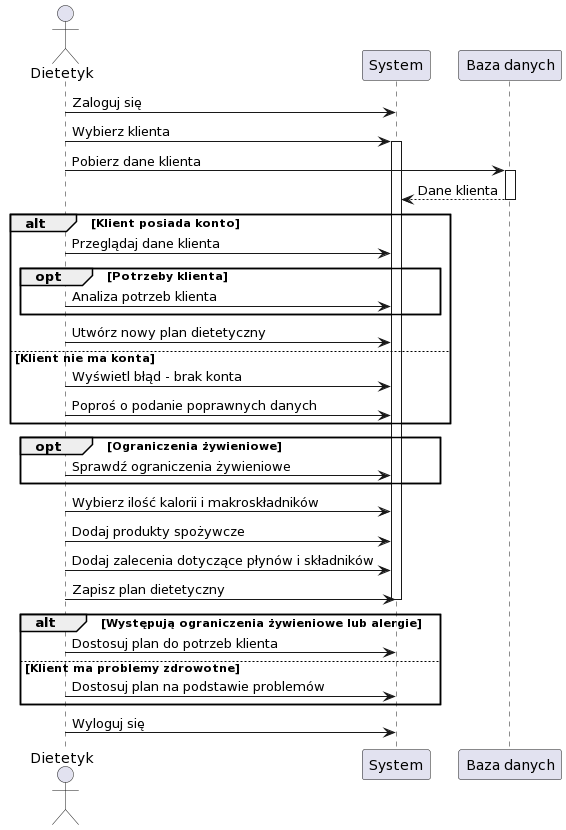
\includegraphics{diagrams/sequence/dietetyk_stworz_plan}}

{Aktorzy biorący udział: Dietetyk}

{Cel przypadku: Utworzenie planu dietetycznego dla klienta}

{Warunki początkowe: Dietetyk jest zalogowany do systemu i ma dostęp do
panelu dietetyka. Klient posiada konto w systemie.}

{Warunki końcowe: Utworzony jest nowy plan dietetyczny dla klienta.}

{Główny ciąg zdarzeń:}

\begin{enumerate}
\tightlist
\item
  {Dietetyk wybiera klienta, dla którego chce utworzyć plan
  dietetyczny.}
\item
  {Dietetyk przegląda dane klienta dotyczące jego aktualnej diety, stylu
  życia, celów odchudzania lub przyrostu masy mięśniowej.}
\item
  {Dietetyk tworzy nowy plan dietetyczny, wybierając odpowiednią ilość
  kalorii oraz makroskładników (białka, węglowodany, tłuszcze) dla
  klienta.}
\item
  {Dietetyk dodaje odpowiednie produkty spożywcze do planu
  dietetycznego.}
\item
  {Dietetyk dodaje zalecenia dotyczące spożycia płynów, witamin i
  minerałów.}
\item
  {Dietetyk zapisuje plan dietetyczny w systemie.}
\end{enumerate}

{Alternatywne ciągi zdarzeń:}

{2a. Jeśli klient nie ma jeszcze konta w systemie, system wyświetla błąd
i prosi o podanie poprawnych danych}

{4a. Jeśli w planie dietetycznym występują ograniczenia żywieniowe lub
alergie, dietetyk dostosowuje plan do potrzeb klienta.}

{5a. Jeśli klient ma problemy zdrowotne, dietetyk konsultuje się z
lekarzem lub innym specjalistą w celu dostosowania planu dietetycznego.}

{}

\begin{enumerate}
\setcounter{enumi}{7}
\tightlist
\item
  {Edytuj plan dietetyczny}
\end{enumerate}

{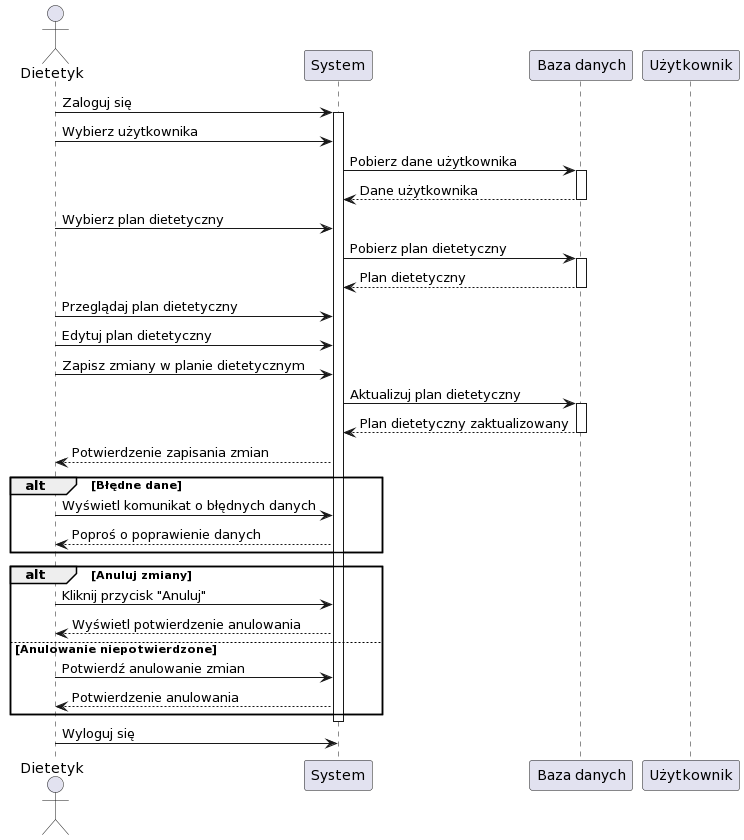
\includegraphics{diagrams/sequence/dietetyk_edytuj_plan.png}}

{Aktorzy biorący udział: Dietetyk}

{Cel przypadku: Edycja planu dietetycznego dla danego użytkownika}

{Warunki początkowe: Dietetyk zalogowany w systemie, wybrany użytkownik
oraz plan dietetyczny}

{Warunki końcowe: Plan dietetyczny dla użytkownika został
zaktualizowany}

{Główny ciąg zdarzeń:}

\begin{enumerate}
\tightlist
\item
  {Dietetyk wybiera użytkownika, dla którego chce edytować plan
  dietetyczny.}
\item
  {Dietetyk wybiera plan dietetyczny, który chce edytować.}
\item
  {System wyświetla istniejący plan dietetyczny dla użytkownika.}
\item
  {Dietetyk wprowadza zmiany w planie dietetycznym (np. zmiana posiłków,
  ilości kalorii).}
\item
  {Dietetyk zapisuje zmiany w planie dietetycznym.}
\item
  {System aktualizuje plan dietetyczny dla wybranego użytkownika.}
\item
  {System wyświetla potwierdzenie zapisania zmian w planie
  dietetycznym.}
\end{enumerate}

{Alternatywne ciągi zdarzeń:}

\begin{itemize}
\tightlist
\item
  {W przypadku błędnie wprowadzonych danych, system wyświetla odpowiedni
  komunikat i prosi o poprawienie wprowadzonych informacji.}
\item
  {Dietetyk może anulować wprowadzone zmiany, klikając przycisk
  "Anuluj". System wyświetla potwierdzenie anulowania zmian lub prosi o
  potwierdzenie przed anulowaniem.}
\end{itemize}

{}

\begin{enumerate}
\setcounter{enumi}{8}
\tightlist
\item
  {Usuń plan dietetyczny}
\end{enumerate}

{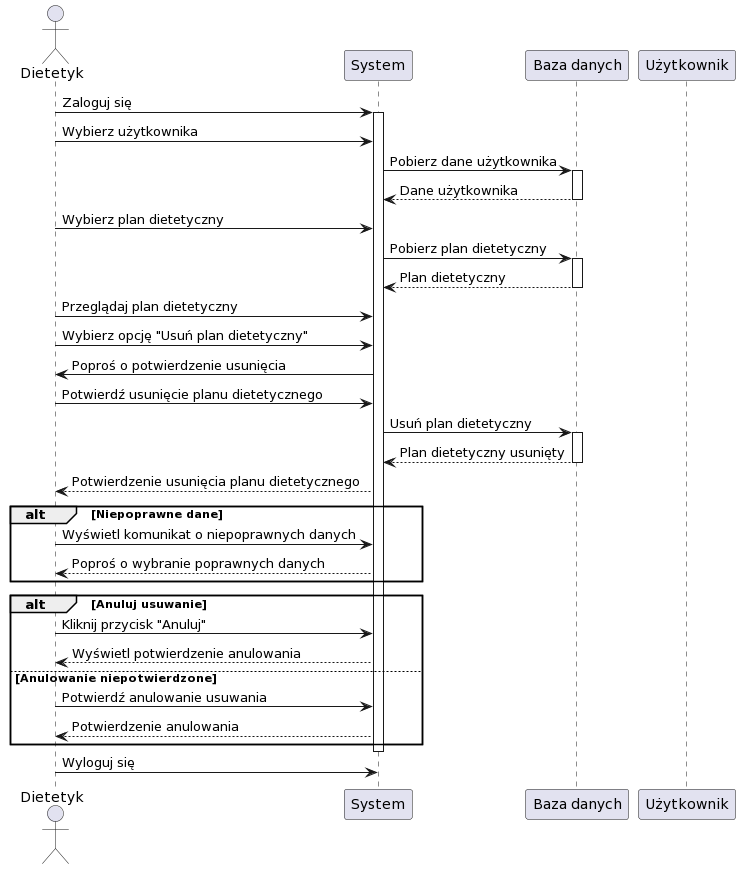
\includegraphics{diagrams/sequence/dietetyk_usun_plan.png}}
{Aktorzy biorący udział: Dietetyk}

{Cel przypadku: Usunięcie planu dietetycznego dla danego użytkownika}

{Warunki początkowe: Dietetyk zalogowany w systemie, wybrany użytkownik
oraz plan dietetyczny}

{Warunki końcowe: Plan dietetyczny dla użytkownika został usunięty}

{Główny ciąg zdarzeń:}

\begin{enumerate}
\tightlist
\item
  {Dietetyk wybiera użytkownika, dla którego chce usunąć plan
  dietetyczny.}
\item
  {Dietetyk wybiera plan dietetyczny, który chce usunąć.}
\item
  {System wyświetla istniejący plan dietetyczny dla użytkownika.}
\item
  {Dietetyk wybiera opcję "Usuń plan dietetyczny".}
\item
  {System prosi o potwierdzenie usunięcia planu dietetycznego.}
\item
  {Dietetyk potwierdza usunięcie planu dietetycznego.}
\item
  {System usuwa plan dietetyczny dla wybranego użytkownika.}
\item
  {System wyświetla potwierdzenie usunięcia planu dietetycznego.}
\end{enumerate}

{Alternatywne ciągi zdarzeń:}

\begin{itemize}
\tightlist
\item
  {W przypadku niepoprawnie wybranego użytkownika lub planu
  dietetycznego, system wyświetla odpowiedni komunikat i prosi o
  wybranie poprawnych danych.}
\item
  {Dietetyk może anulować usuwanie planu dietetycznego, klikając
  przycisk "Anuluj". System wyświetla}
\end{itemize}
